\chapter{Results and Analysis}
\label{chapter:results}

\section{Acceleration of Post-Quantum Key Encapsulation Mechanisms}

\todo[inline]{
What specialized instructions and features applicable for post-quantum keyencapsulationmechanisms are available in z15 and how are they used in context?
}

This section studies the \gls{nist} submissions' underlying mathematics, the authors' own optimizations as well as relevant literature on cryptography optimization.

\subsection{Identifying Hot Paths}
\label{section:results:hot-paths}

The following sections analyzes the \gls{ntru} and \gls{mceliece} submissions to the \gls{nist} standardization process, in terms of the reference implementations and what branches the code takes, how many times they are taken, as well as how many instructions are retired in each function. Unless otherwise stated, the measurements are the percentage of instructions performed in a function or in a line of code, relative to the parent.

All of the data as well as further visualizations not included in this work is published on GitHub\footnote{\href{https://github.com/profiling-pqc-kem-thesis/data}{https://github.com/profiling-pqc-kem-thesis/data}}.

\subsubsection{NTRU}

The \gls{ntru} reference implementations consists of three API methods - keypair generation via \textit{crypto\_kem\_keypair}, encryption (encapsulation) via \textit{crypto\_kem\_enc} and decryption (decapsulation) via \textit{crypto\_kem\_dec}  decryption (decapsulation). These API functions may in turn call several internal functions, such as the polynomial math library which functions are prefixed \textit{poly\_}.

The following graphs contain relative measurements denoting the percentage of instructions spent in each method. Both the HPS and HRSS variants of \gls{ntru} perform alike, hence only one set of graphs is shown for \gls{ntru} as a whole.

Figure \ref{figure:result:hot-paths:ntru:crypto_kem_keypair} shows us that $40\%$ of the instructions of generating a key-pair is spent in the library function \textit{poly\_Rq\_mul} - a function which multiplies two polynomials in $\mathbb{R}^q$. Another $20\%$ of the instructions are spent on inverting a polynomial in $\mathbb{R}^2$ - in \textit{poly\_R2\_inv}. In total, the polynomial math accounts for at least $60\%$ of the time spent on generating a keypair.

\begin{figure}[H]
    \centering
    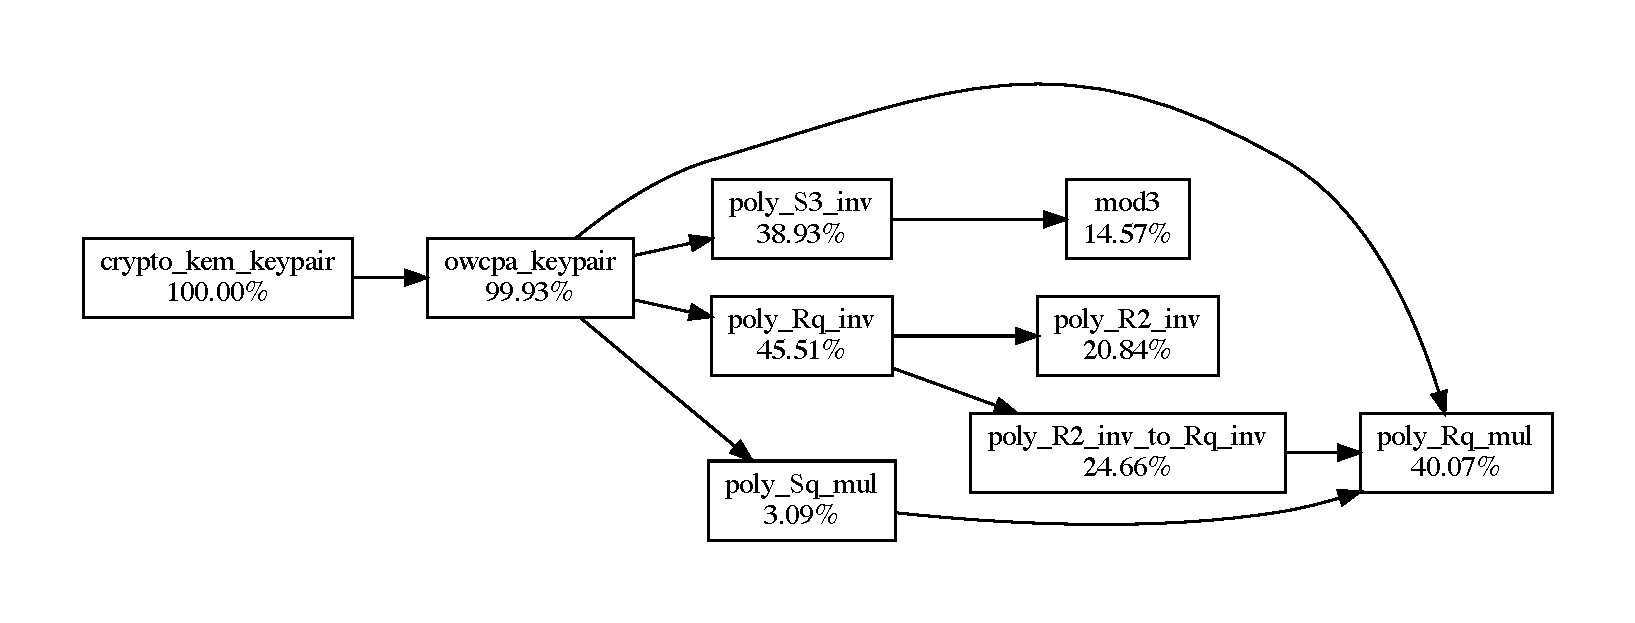
\includegraphics[width=15cm, height=10cm, keepaspectratio]{chapters/results/hot-paths/ntru/crypto_kem_keypair.pdf}
    \caption{Relative instruction count of \gls{ntru}'s \textit{crypto\_kem\_keypair}}
    \label{figure:result:hot-paths:ntru:crypto_kem_keypair}
\end{figure}

Figure \ref{figure:result:hot-paths:ntru:crypto_kem_enc} describes the encapsulation API function. The key is generated using random bytes which are fed through 256-bit \gls{aes} in its Electronic Code Book (ECB) configuration to produce uniformly random bytes. Again, we see a significant percentage of the instructions spent in the polynomial library - in \textit{poly\_Rq\_mul}.

\begin{figure}[H]
    \centering
    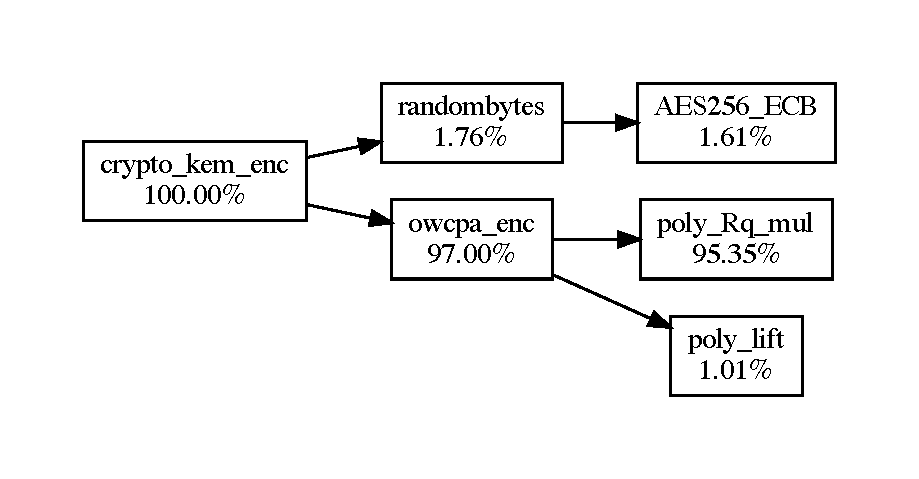
\includegraphics[width=15cm, height=10cm, keepaspectratio]{chapters/results/hot-paths/ntru/crypto_kem_enc.pdf}
    \caption{Relative instruction count of \gls{ntru}'s \textit{crypto\_kem\_keypair}}
    \label{figure:result:hot-paths:ntru:crypto_kem_enc}
\end{figure}

The decryption function of \gls{ntru} is presented in figure \ref{figure:result:hot-paths:ntru:crypto_kem_dec}. Virtually all of the instructions spent decrypting (decapsulating) a key is spent in the \textit{poly\_Rq\_mul} function.

\begin{figure}[H]
    \centering
    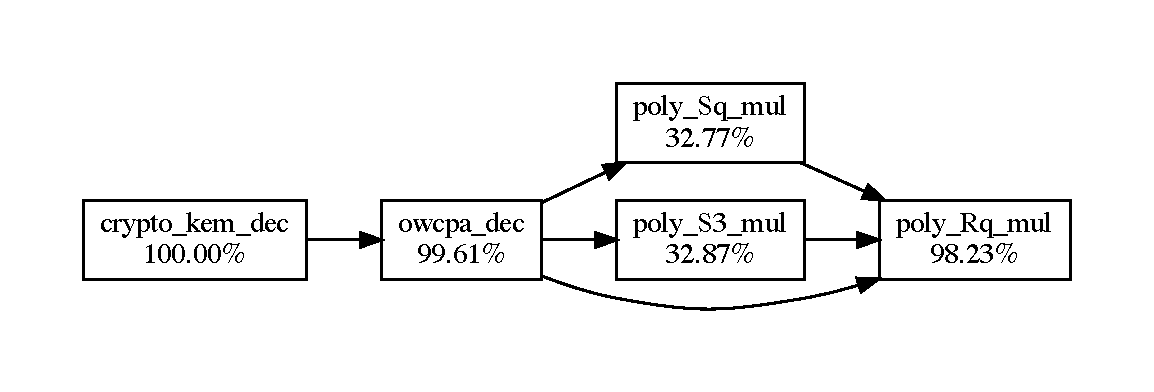
\includegraphics[width=15cm, height=10cm, keepaspectratio]{chapters/results/hot-paths/ntru/crypto_kem_dec.pdf}
    \caption{Relative instruction count of \gls{ntru}'s \textit{crypto\_kem\_dec}}
    \label{figure:result:hot-paths:ntru:crypto_kem_dec}
\end{figure}

Looking at the code of \textit{poly\_Rq\_mul} as shown in figure \ref{figure:result:hot-paths:ntru:poly_Rq_mul}, it is evident that the vast majority of instructions are spent on multiplying and adding numbers in loops. The value of \textit{NTRU\_N} corresponds to the parameter set. For \gls{ntru} HRSS 701, the value is 701 and for \gls{ntru} HPS 4096821 the value is 821.

\begin{figure}[H]
    \centering
    \begin{lstlisting}[language=C]
void poly_Rq_mul(poly *r, const poly *a, const poly *b) {
  int k, i;

  for (k = 0; k < NTRU_N; k++) {
    r->coeffs[k] = 0;
    for (i = 1; i < NTRU_N - k; i++) // 10.21%
      r->coeffs[k] += a->coeffs[k + i] * b->coeffs[NTRU_N - i]; // 42.75%
    for (i = 0; i < k + 1; i++) // 8.20%
      r->coeffs[k] += a->coeffs[k - i] * b->coeffs[i]; // 38.79%
  }
}
    \end{lstlisting}
    \caption{Annotated source code of \gls{ntru}'s \textit{poly\_Rq\_mul}}
    \label{figure:result:hot-paths:ntru:poly_Rq_mul}
\end{figure}

To summarize, it is shown that factors such as the speed of \gls{aes} has little to do with the overall performance of the algorithm. Furthermore, it seems as if the polynomial library functions account for the vast majority of instructions spent on key-pair generation, encryption and decryption. The function \textit{poly\_Rq\_mul}, which multiplies two polynomials in $\mathbb{R}^q$), accounts for most of the calculations performed.

\subsubsection{Classic McEliece}
The \gls{mceliece} reference implementation consists of three API methods - \textit{crypto\_kem\_keypair}, \textit{crypto\_kem\_enc} and \textit{crypto\_kem\_dec} for key-pair generation, encryption (encapsulation) and decryption (decapsulation), respectively. These API functions may in turn call several internal functions. We will only present the hot-paths for the \gls{mceliece} 8192128 non-f variant because it can quite accurately represent the hot-paths for all \gls{mceliece} variants. In the appendix, all hot-paths can be found. 

In figure \ref{figure:result:hot-paths:classic-mceliece:crypto_kem_keypair}, we can see the \textit{crypto\_kem\_keypair} function and its only significant internal function, the \textit{pk\_gen} function that takes up 98.57\% of the execution time. In figure \ref{figure:result:hot-paths:classic-mceliece:pk_gen}, we can see the deeper look into the \textit{pk\_gen} function there we can see that all its internal functions and that they do not make up much of the instructions. Most of the instructions are inside of the \textit{pk\_gen} function itself.\todo{explain better}

\begin{figure}[H]
    \centering
    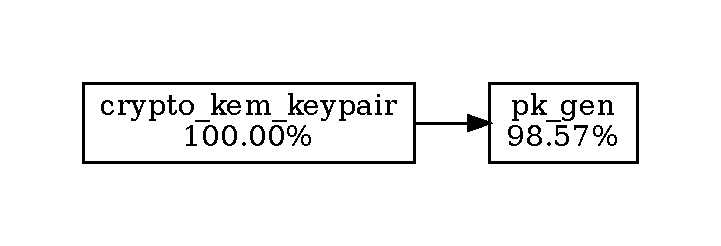
\includegraphics[width=15cm, height=10cm, keepaspectratio]{chapters/results/hot-paths/classic-mceliece/8192128/crypto_kem_keypair.pdf}
    \caption{Relative instruction count of \gls{mceliece}'s \textit{crypto\_kem\_keypair}}
    \label{figure:result:hot-paths:classic-mceliece:crypto_kem_keypair}
\end{figure}

\begin{figure}[H]
    \centering
    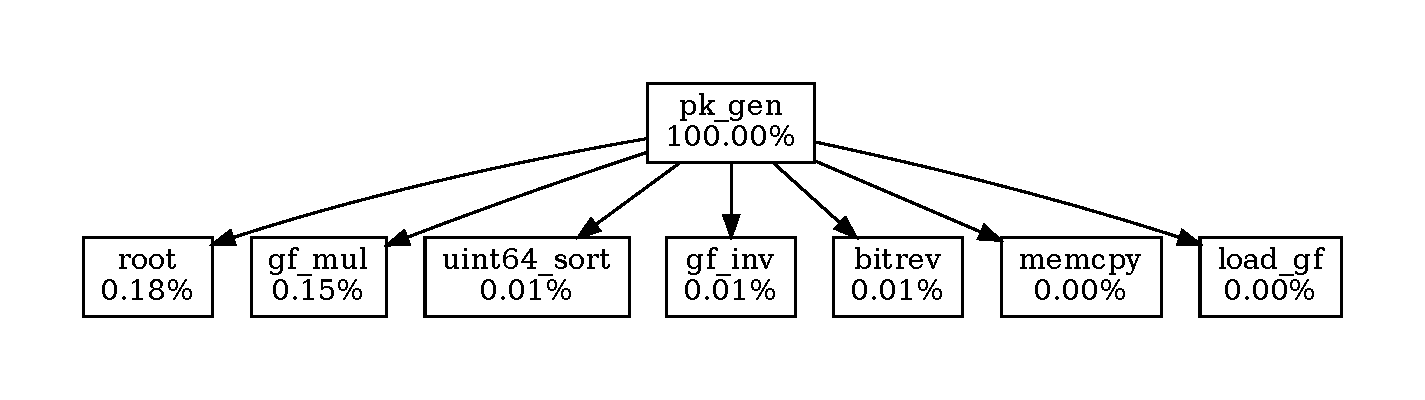
\includegraphics[width=15cm, height=10cm, keepaspectratio]{chapters/results/hot-paths/classic-mceliece/8192128/pk_gen.pdf}
    \caption{Relative instruction count of \gls{mceliece}'s \textit{pk\_gen}}
    \label{figure:result:hot-paths:classic-mceliece:pk_gen}
\end{figure}

\begin{figure}[H]
    \centering
    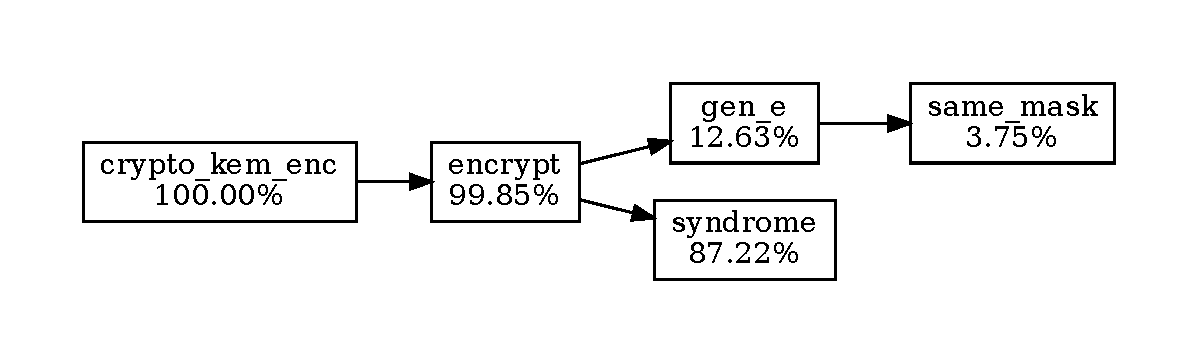
\includegraphics[width=15cm, height=10cm, keepaspectratio]{chapters/results/hot-paths/classic-mceliece/8192128/crypto_kem_enc.pdf}
    \caption{Relative instruction count of \gls{mceliece}'s \textit{crypto\_kem\_keypair}}
    \label{figure:result:hot-paths:classic-mceliece:crypto_kem_enc}
\end{figure}

\begin{figure}[H]
    \centering
    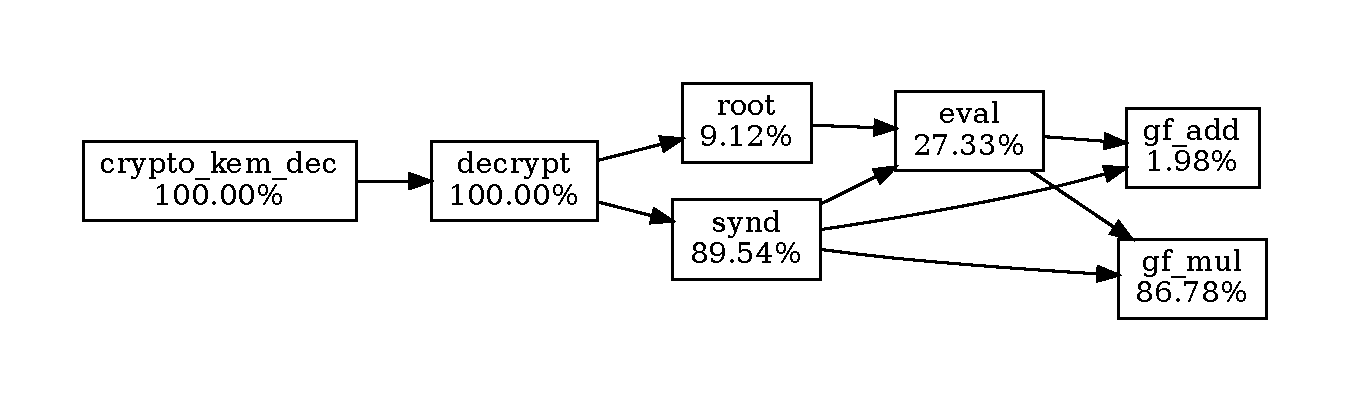
\includegraphics[width=15cm, height=10cm, keepaspectratio]{chapters/results/hot-paths/classic-mceliece/8192128/crypto_kem_dec.pdf}
    \caption{Relative instruction count of \gls{mceliece}'s \textit{crypto\_kem\_dec}}
    \label{figure:result:hot-paths:classic-mceliece:crypto_kem_dec}
\end{figure}

\todo[inline]{Var tydliga med hot paths och tid. Exempelvis så lär diagrammet för pk\_gen visa 0\% för vissa funktioner så som root, men om vi ser till hot paths så lär vi se att de kallas flera miljoner gånger. Kanske ha en graf som visar antalet invocations?}

\todo[inline]{Ingen microbenchmark för eval, gf\_mul och gf\_add - de körs så många gånger att overheaden för profiling blev 1000x. McEliece kallar på många många tusen funktioner (hundra tusen, uppemot miljoner?) - det i sig bör ge mer overhead. }

\section{Post-Quantum Cryptography on z15}

\todo[inline]{
What specialized instructions and features applicable for post-quantum keyencapsulation mechanisms are available in z15 and how are they used in context?

Litteraturstudien.
}

\section{The Performance of Post-Quantum Key Exchange Mechanisms}

This section presents the results of the experiment as outlined in section \ref{section:method:experiment}. It further discusses the performance of \gls{post-quantum} \glspl{kem} and how they may differ on various architectures and hardware.

\subsection{Algorithm Performance}

In section \ref{section:method:experiment:phase1:implementation-configurations} it was written that the monitored functions for the micro benchmark would be based off of data found in the hot paths analysis. In the end, the functions presented in Table \ref{table:results:performance:micro-functions} were monitored during the micro benchmark. Note that although the randombytes function is available in both \gls{ntru} and \gls{mceliece}, it was found in section \ref{section:results:hot-paths} to not be significant enough to warrant further analysis.

\begin{table}[H]
    \centering
    \caption{Monitored Functions}
    \label{table:results:performance:micro-functions}
    \begin{tabularx}{\linewidth}{l X}
        \toprule
        \thead{Name} & \thead{Description} \\
        \midrule
        \multicolumn{3}{c}{\thead[l]{\gls{mceliece} and \gls{ntru}}} \\
        %\midrule
        crypto\_kem\_keypair & Generate a keypair \\
        crypto\_kem\_enc & Generate and encapsulate a key \\
        crypto\_kem\_dec & Decapsulate an encapsulated key \\
        \multicolumn{3}{c}{\thead[l]{\gls{mceliece}}} \\
        pk\_gen & \\
        gen\_e & \\
        syndrome & \\
        % syndrome\_asm & The same as syndrome, but implemented in assembly targeting AVX2\\
        root & \\
        synd & \\
        \multicolumn{3}{c}{\thead[l]{\gls{ntru}}} \\
        poly\_Rq\_mul & Multiply a polynomial with another in $\mathbb{R}_q$\\
        poly\_S3\_inv & Invert a polynomial in $\mathbb{S}_3$\\
        randombytes & Retrieve uniformly random bytes \\
        poly\_Rq\_inv & Invert a polynomial in $\mathbb{R}_2$\\
        poly\_R2\_inv & Invert a polynomial in $\mathbb{R}_2$\\
        poly\_R2\_inv\_to\_Rq\_inv & Lift an inverted polynomial from $\mathbb{R}_2$ to $\mathbb{R}_q$ \\
        poly\_Sq\_mul & Multiply a polynomial in $\mathbb{S}_q$ with another\\
        \bottomrule
    \end{tabularx}
\end{table}

\todo[inline]{
Does the performance of post-quantum key encapsulation mechanisms differ between architectures and if so, how?
What techniques may be used to increase the performance of post-quantum key encapsulation mechanisms?
}

\todo[inline]{
Talk about all the sequential data here - sequential, heap, micro, stack. Use all data, no matter the underlying system, to get an average of the state of the machines? If we only use relative measurements, that will be fine even though the i3 may lower the throughput?
}

\subsection{Hardware Performance}

\todo[inline]{
Does the performance of post-quantum key encapsulation mechanisms differ between architectures and if so, how?
What techniques may be used to increase the performance of post-quantum key encapsulation mechanisms?
}

\todo[inline]{
Talk about the parallel benchmark here, hardware throughput, hardware differences.
}

\subsection{Memory Usage}

As outlined in the method, section \ref{section:method:experiment:phase1:measurements}, we measured the heap usage of the algorithms by monitoring heap allocation and deallocation methods such as malloc using the tool heaptrack. We found that the heap allocation did not change across environments nor between the analyzed optimizations except for some few occurances. As for the implementations, this is rather unsurprising as changing how the allocations worked would alter the behavior of the code. As we found that the heap behavior of the algorithms were consistent throughout our test, we will for the rest of this section not refer\todo{No longer true?} to any specific environment or optimization used for the algorithms unless otherwise noted. When talking about allocation, we will refer to the peak allocation - that is, the maximum allocated bytes recorded during a function's lifetime.

At one point, the \gls{ntru} implementations allocated $264$ bytes generating a keypair. These bytes were allocated by OpenSSL to initialize the library's envelope suite of functions. In context, this is done as the \gls{ntru} implementation uses OpenSSL's \gls{aes} ECB implementation to generate uniform pseduo-random bytes. The invocation of the \gls{aes} function itself resulted in $168 + 40$ bytes being allocated by the OpenSSL \gls{aes} ECB implementation. Beyond these bytes, the \gls{ntru} implementation did not require any additional heap allocation during its runtime. It's important to note, however, that the algorithm relies on additional memory in the form of parameters given to the implementation\todo{Remove this part and talk about the parameters seperately and discuss the authors' results as well}.

Just like the \gls{ntru} implementations, the \gls{mceliece} implementations make use of OpenSSL to create uniform pseudo-random bytes. As such, the same $264$ bytes are allocated to initialize OpenSSL's envelope suite of functions, as well as the $168 + 40$ bytes to actually encrypt random data to produce a uniformly distributed series of bytes. No further allocations were found to be made.

The \gls{ecdhe} and \gls{dhe} implementations are based entirely on functions made available by OpenSSL. All of the implementations had an increase in the number of allocations made. The \gls{dhe} implementation in the IBM Community Cloud environment saw an allocation of $16960$ bytes during keypair generation made from a constant-time modulo exponentiation on an arbitrary large number. All other environments allocated $9024$ bytes for the same invocation. Furthermore, the keypair generation saw the allocation of a further $1024$ bytes in the IBM Community Cloud environment seemingly related to the same modulo operation.
The operation of dividing an integer was found to correlate to an additional $536$ bytes in the Cloud Provider 1 environment and $528$ bytes in all of the other environments. The environments saw an additional $520 + 512 + 400$ bytes corresponding to the dealing of arbitrary large numbers whilst generating a keypair. Fetching random data raised the allocation with $360 + 272$ bytes in all environments except the Cloud Provider 1, which saw an allocation of $352 + 280$ bytes instead. There were further allocations made, all of which are summarized in Table \ref{table:results:memory:dhe-heap}. The \gls{ecdhe} implementation behaved much like the \gls{dhe}, with the peaks differing between some environments. The implementation too worked with arbitrary numbers and as such had several of the same allocations as the \gls{dhe} implementations. The peaks are presented in Table \ref{table:results:memory:ecdhe-heap}.


\begin{table}
    \centering
    \caption{Heap Allocation in Bytes for \gls{dhe}}
    \label{table:results:memory:deh-heap}
    \begin{tabularx}{\linewidth}{X c c c}
        \toprule
        \thead{Environment} & \thead{OpenSSL Version} & \multicolumn{2}{c}{\thead{Sum of Peaks}}\\
        & & \thead{Keypair} & \thead{Exchange} \\
        \midrule
        IBM Community Cloud & 1.1.1g FIPS & 19772 & 19248 \\
        Cloud Provider 1 & 1.1.1 & 12076 & 12080 \\
        Cloud Provider 2 & 1.1.1f & 11852 & 11536\\
        Modern Workstation & 1.1.1f & 11852 & 11536 \\
        Modern Laptop & 1.1.1f & 11852 & 11536 \\
        Old Mid-Range Laptop & 1.1.1f & 11852 & 11536\\
        Old Low-Range Laptop & 1.1.1f & 11852 & 11536\\
        \bottomrule
    \end{tabularx}
\end{table}
\todo{correct values in table}

\begin{table}
    \centering
    \caption{Heap Allocation in Bytes for \gls{ecdhe}}
    \label{table:results:memory:ecdhe-heap}
    \begin{tabularx}{\linewidth}{X c c c c}
        \toprule
        \thead{Environment} & \thead{Curve} & \thead{OpenSSL Version} & \multicolumn{2}{c}{\thead{Sum of Peaks}}\\
        & & & \thead{Keypair} & \thead{Exchange} \\
        \midrule
        IBM Community Cloud & P-256 & 1.1.1g FIPS & 4920 & 1520 \\
        IBM Community Cloud & 25519 & 1.1.1g FIPS & 4524 & 1520 \\

        Cloud Provider 1 & P-256 & 1.1.1 & - & - \\
        Cloud Provider 1 & 25519 & 1.1.1 & - & - \\

        Cloud Provider 2 & P-256 & 1.1.1f & 2584 & 2136 \\
        Cloud Provider 2 & 25519 & 1.1.1f & 1192 & 2005\\

        Modern Workstation & P-256 & 1.1.1f & 2584 & 2136 \\
        Modern Workstation & 25519 & 1.1.1f & 1192 & 2005 \\
        
        Modern Laptop & P-256 & 1.1.1f & 2584 & 2136 \\
        Modern Laptop & 25519 & 1.1.1f & 1192 & 2005 \\
        
        Old Mid-Range Laptop & P-256 & 1.1.1f & 2584 & 2136\\
        Old Mid-Range Laptop & 25519 & 1.1.1f & 1192 & 2005\\
        
        Old Low-Range Laptop & P-256 & 1.1.1f & 2584 & 2136\\
        Old Low-Range Laptop & 25519 & 1.1.1f & 1192 & 2005\\
        \bottomrule
    \end{tabularx}
\end{table}
\todo{correct values in table}

In terms of stack usage, the results vary between the implementations, compilers and features. For instance, the polynomial math function poly\_Rq\_mul in \gls{ntru}, which was identified as constituting most of the time spent in the algorithm, varies between taking up $70499$ and $188$ bytes. In all environments, the HPS 4096821 AVX2 variant takes up $70499$ bytes. This does not change between compilers or optimization flags, which could be due to the fact that the implementation is written in assembly - leaving little room for the compiler to optimize for size. The same goes for the HRSS 701 variant of \gls{ntru} - the size is consistently $55317$ across environments and optimization flags. The lowest sizes are found when the reference implementation is compiled with optimization. The sizes are presented in Table \ref{table:results:memory:ntru-stack}. Although the optimization flags used were not chosen for improving the size of the binary, the size of the function has been lowered in all cases. Although the same version of GCC was used for several environments, the results differed between $188$ and $192$ bytes. Clang continually produced larger regions than GCC. Furthermore, more recent versions of the compilers seem to have produced smaller sizes.

\begin{table}
    \centering
    \caption{Stack Size of poly\_Rq\_mul in Bytes for the Optimized Reference Implementation}
    \label{table:results:memory:ntru-stack}
    \begin{tabularx}{\linewidth}{X c c c c}
        \toprule
        \thead{Environment} & \thead{Compiler} & \thead{Compiler Version} & \thead{Optimized Size} & \thead{Reference Size}\\
        \midrule
        Cloud Provider 1 & clang & 6.0.0 & 702 & N/A \\
        IBM Community Cloud & clang & 10.0.1 & 522 & N/A \\
        Cloud Provider 2 & clang & 10.0.0 & 380 & N/A \\
        Modern Laptop & clang & 10.0.0 & 380 & N/A \\
        Modern Workstation & clang & 10.0.0 & 380 & N/A \\
        Cloud Provider 2 & clang & 10.0.0 & 380 & N/A \\
        Modern Laptop & clang & 10.0.0 & 380 & N/A \\
        Old Low-Range Laptop & clang & 10.0.0 & 300 & N/A \\
        Old Mid-Range Laptop & clang & 10.0.0 & 300 & N/A \\
    
        IBM Community Cloud & gcc & 8.3.1 & 242 & 382 \\
        Old Low-Range Laptop & gcc & 9.3.0 & 196 & 255 \\
        Old Mid-Range Laptop & gcc & 9.3.0 & 196 & 255 \\
        Cloud Provider 1 & gcc & 7.5.0 & 192 & 253\\
        Cloud Provider 2 & gcc & 9.3.0 & 188 & 255\\
        Modern Laptop & gcc & 9.3.0 & 188 & 255\\
        Modern Workstation & gcc & 9.3.0 & 188 & 255\\
        \bottomrule
    \end{tabularx}
\end{table}

The same correlation between optimization flags and compiler versions could not be found in the case of \gls{mceliece} and pk\_gen. In that case, the largest recorded size was found in IBM Community Cloud's optimized reference implementation with $22858$ bytes. The optimized AVX2 implementation of the Modern Workstation and Modern Laptop came second with $22123$ bytes. Lastly, the smallest size recorded was found in the optimized reference implementation of Old Mid-Range Laptop and Old Low-Range Laptop at $2026$ bytes.

As for other functions of the \glspl{kem}, the data is too massive to comprehensively refer to here. There are, however, tables in the appendix for average sizes as compared to the reference implementation compiled with GCC. In Table \ref{table:result:ntru-average-stack-increase-cloud}, for example, one can see that Clang seems to produce smaller binaries. Furthermore, the optimized AVX2 build results in the largest binaries - with symbols taking 8-10 times the size of the reference implementation.

\todo[inline]{Discuss stack usage of ECDHE, DHE?}

The measurements presented up until this point have been related to either the runtime behavior of the algorithms, or the static requirements they place on the environment. These measurements have not included the parameters fed to the algorithms - which could affect real-world applications. The remaining part of this section will present data gathered from the various implementations.

The \glspl{kem} tested conform to the same API. Their signatures are presented in figure \ref{figure:result:memory:kem-api}. The function crypto\_kem\_keypair, which generates a keypair takes in a public key and a secret key. The encapsulation function, crypto\_kem\_enc, takes in a ciphertext buffer, a key buffer and the public key of a peer. Lastly, the decapsulation function, crypto\_kem\_dec takes in a key buffer, the ciphertext as received from a peer and the secret key. The sizes of these parameters differ between algorithms and implementations - but is not changed depending on the environment or optimizations. Table \ref{table:results:memory:kem-parameter-sizes} shows the sizes of the parameters in bytes. The sizes do not differ between the "f" variants of \gls{mceliece}. Therefore only two variants of \gls{mceliece} are presented.

\begin{figure}
    \centering
    \begin{lstlisting}[language=C]
int crypto_kem_keypair(unsigned char *public_key, unsigned char *private_key);
int crypto_kem_enc(unsigned char *ciphertext, unsigned char *key, const unsigned char *public_key);
int crypto_kem_dec(unsigned char *key, const unsigned char *ciphertext, const unsigned char *private_key);
    \end{lstlisting}
    \caption{The API of the \gls{kem} Implementations}
    \label{figure:result:memory:kem-api}
\end{figure}

\begin{table}
    \centering
    \caption{Parameter Sizes in Bytes of the \glspl{kem} Under Test}
    \label{table:results:memory:kem-parameter-sizes}
    \begin{tabularx}{\linewidth}{X c c c c c}
        \toprule
        \thead{Algorithm} & \thead{Parameters} & \thead{public\_key} & \thead{private\_key} & \thead{ciphertext} & \thead{key}\\
        \midrule
        \gls{mceliece} & 8192128(f) & 1357824 & 14120 & 240 & 32 \\
        \gls{mceliece} & 6960119(f) & 1047319 & 13948 & 226 & 32 \\
        \gls{ntru} & HRSS 701 & 1138 & 1450 & 1138 & 32 \\
        \gls{ntru} & HPS 4096821 & 1230 & 1590 & 1230 & 32 \\
        \bottomrule
    \end{tabularx}
\end{table}

The APIs are similar, but not the same for the \gls{kex} implementations. That is due to \gls{dh} requiring the so called Diffie-Hellman Parameters $p$ and $g$. The APIs are shown in figure \ref{figure:results:memory:kex-api}. As with the \gls{kem} implementations, the \gls{kex} implementations use two buffers for a public and a private key when generating a keypair. The \gls{dh} implementation also requires the previously mentioned domain parameters $p$ and $g$ - both buffers of bytes containing the respective parameter. The crypto\_dh\_enc functions further use a key buffer. There is no analogous ciphertext as the \glspl{kex} are fundamentally different from the \glspl{kem} as covered in \ref{section:background:diffie-hellman}. The sizes of the parameters are presented in Table \ref{table:results:memory:kex-parameter-sizes}.

\begin{figure}
    \centering
    \begin{lstlisting}[language=C]
// Diffie-Hellman
int crypto_dh_keypair(unsigned char *public_key, unsigned char *private_key, unsigned char *p, unsigned char *g);

// Diffie-Hellman
int crypto_dh_enc(unsigned char *key, const unsigned char *private_key, const unsigned char *public_key, unsigned char *p, unsigned char *g);

// Elliptic-Curve Diffie-Hellman
int crypto_dh_keypair(unsigned char *public_key, unsigned char *private_key);

// Elliptic-Curve Diffie-Hellman
int crypto_dh_enc(unsigned char *key, const unsigned char *private_key, const unsigned char *public_key);
    \end{lstlisting}
    \caption{The API of the \gls{kex} Implementations}
    \label{figure:results:memory:kex-api}
\end{figure}

\begin{table}
    \centering
    \caption{Parameter Sizes in Bytes of the \glspl{kex} Under Test}
    \label{table:results:memory:kex-parameter-sizes}
    \begin{tabularx}{\linewidth}{X c c c c c c}
        \toprule
        \thead{Algorithm} & \thead{Parameters} & \thead{public\_key} & \thead{private\_key} & \thead{$p$} & \thead{$g$} & \thead{key}\\
        \midrule
        \gls{dh} & 2048    &255 & 255 & 256  & 1 & 32 \\
        \gls{ecdh} & P-256 & 65 & 32 & - & - & 32 \\
        \gls{ecdh} & 25519 & 32 & 32 & - & - & 32 \\
        \bottomrule
    \end{tabularx}
\end{table}

\section{Throughput Performance}

As outlined in section \ref{section:method:experiment:phase2}, the throughput of the algorithms in each environment under test was evaluated for a series of parallelism configurations. The initial plan was to use the best-performing algorithm for each environment, as identified by the sequential benchmarks. Early results, however, were not conclusive and we therefore ended up running the parallel benchmarks on both GCC and Clang builds of the best-performing variant. The throughput of the algorithms differed depending on the environment and compiler used. The lowest throughput was found in Clang builds in the Old Low-Range Laptop, for which runs are presented in figure \ref{figure:results:throughput:mceliece:old-low-range-laptop} and figure \ref{figure:results:throughput:ntru:old-low-range-laptop}. As can be seen in figure \ref{figure:results:throughput:mceliece:old-low-range-laptop}, Clang yielded down to one fifth of the encryption throughput of the comparable GCC build, but also resulted in a roughly 5\% speedup over the comparable GCC implementation. The \gls{ntru} tests, as presented in figure \ref{figure:results:throughput:ntru:old-low-range-laptop}, Clang produced a 50\% lower keypair throughput, 20\% lower encryption and decryption throughput than comparable versions compiled with GCC. A similar difference in throughput was also found in the Old Mid-Range Laptop and the IBM Community Cloud environments.

\begin{figure}
    \centering
    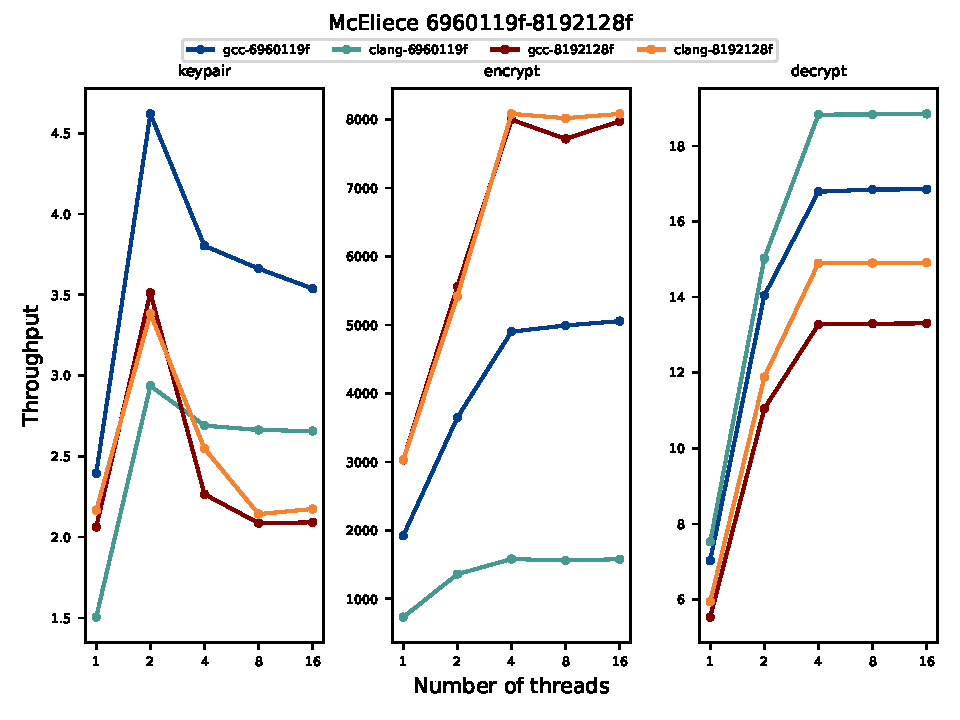
\includegraphics[scale=0.75]{chapters/results/throughput/McEliece 6960119f-8192128f Old Low-Range Laptop.pdf}
    \caption{Throughput of \gls{mceliece} on Old Low-Range Laptop}
    \label{figure:results:throughput:ntru:old-low-range-laptop}
\end{figure}

\begin{figure}
    \centering
    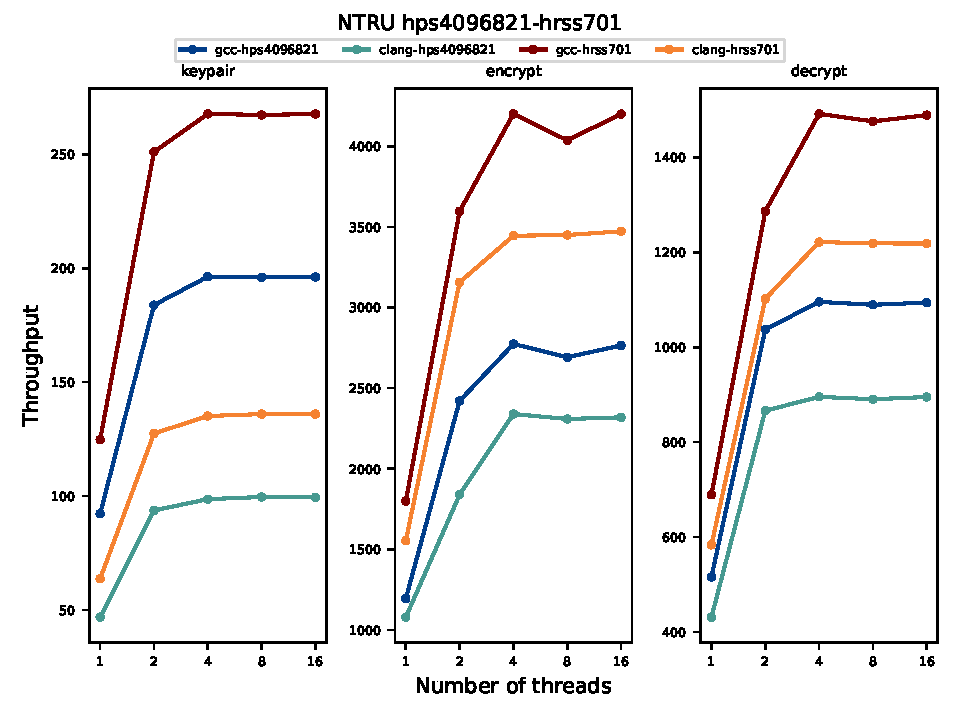
\includegraphics[scale=0.75]{chapters/results/throughput/NTRU hps4096821-hrss701 Old Low-Range Laptop.pdf}
    \caption{Throughput of \gls{mceliece} on Old Low-Range Laptop}
    \label{figure:results:throughput:mceliece:old-low-range-laptop}
\end{figure}

\section{Lekhörna}

\begin{table}[H]
    \centering
    \caption{Parallel Throughput Runs for ntru hrss701 (keypair)}
    \begin{tabularx}{\linewidth}{X c c c c c c c c c c}
        \toprule
        \thead{Environment} & \thead{Compiler} & \multicolumn{7}{c}{\thead{Threads}}\\
        & & 1 & 2 & 4 & 8 & 16 & 32 & 64 & \\
        \midrule
        \multirowcell{4}{Cloud\\ Provider 1}
        & \multirow{2}{*}{gcc} & 10021 & 15345 & 21810 & 22629 & 22963 & 7352\\
        & & N/A & 54\% & 119\% & 128\% & 131\% & -25\%\\
        
        \cmidrule[0.05em](){3-10}
        
        & \multirow{2}{*}{clang} & 9918 & 20027 & 22637 & 22997 & 23753 & 23753\\
        & & N/A & 101\% & 128\% & 131\% & 139\% & 139\%\\
        \bottomrule
        \end{tabularx}
    \end{table}

    \begin{table}[H]
        \centering
        \caption{Parallel Throughput Runs for ntru hrss701 (keypair)}
        \begin{tabularx}{\linewidth}{l c c c c c c c c c c}
            \toprule
            \thead{Environment} & \thead{Compiler} & \multicolumn{7}{c}{\thead{Threads}}\\
            & & 1 & 2 & 4 & 8 & 16 & 32 & 64 &\\
            \midrule
\multirow{4}{*}{Cloud Provider 1} & 
\multirow{2}{*}{gcc} & 10021 & 15345 & 21810 & 22629 & 22963 & & N/A & 53\% & 117\% & 125\% & 129\% & \\
\cmidrule[0.05em](){3-10} & 
\multirow{2}{*}{clang} & 9918 & 20027 & 22637 & 22997 & 23753 & &  & 99\% & 125\% & 129\% & 137\%\\
            \midrule
\multirow{4}{*}{Cloud Provider 2} & 
\multirow{2}{*}{gcc} & 7805 & 10185 & 13663 & 13696 & & N/A & 30\% & 75\% & 75\% & \\
\cmidrule[0.05em](){3-10} & 
\multirow{2}{*}{clang} & 7352 & 12770 & 13289 & 11005 & &  & 63\% & 70\% & 41\%\\
            \midrule
\multirow{4}{*}{IBM Community Cloud} & 
\multirow{2}{*}{gcc} & 137 & 277 & 273 & 275 & & N/A & 101\% & 98\% & 100\% & \\
\cmidrule[0.05em](){3-10} & 
\multirow{2}{*}{clang} & 113 & 226 & 223 & 225 & &  & 64\% & 62\% & 63\%\\
            \midrule
\multirow{4}{*}{Modern Laptop} & 
\multirow{2}{*}{gcc} & 7061 & 12686 & 20221 & 33444 & 36381 & 40489 & & N/A & 79\% & 186\% & 373\% & 415\% & 473\% & \\
\cmidrule[0.05em](){3-10} & 
\multirow{2}{*}{clang} & 5216 & 12854 & 26546 & 35160 & 38757 & 39734 & &  & 82\% & 275\% & 397\% & 448\% & 462\%\\
            \midrule
\multirow{4}{*}{Modern Workstation} & 
\multirow{2}{*}{gcc} & 9256 & 18275 & 36193 & 77144 & 104379 & 103050 & 131102 & & N/A & 97\% & 291\% & 733\% & 1027\% & 1013\% & 1316\% & \\
\cmidrule[0.05em](){3-10} & 
\multirow{2}{*}{clang} & 8771 & 26758 & 35118 & 85408 & 99441 & 101059 & 123903 & &  & 189\% & 279\% & 822\% & 974\% & 991\% & 1238\%\\
            \midrule
\multirow{4}{*}{Old Low-Range Laptop} & 
\multirow{2}{*}{gcc} & 124 & 251 & 267 & 267 & 267 & & N/A & 101\% & 114\% & 114\% & 114\% & \\
\cmidrule[0.05em](){3-10} & 
\multirow{2}{*}{clang} & 63 & 127 & 135 & 135 & 135 & &  & 2\% & 8\% & 8\% & 8\%\\
            \midrule
\multirow{4}{*}{Old Mid-Range Laptop} & 
\multirow{2}{*}{gcc} & 159 & 299 & 319 & 320 & 320 & & N/A & 88\% & 100\% & 101\% & 101\% & \\
\cmidrule[0.05em](){3-10} & 
\multirow{2}{*}{clang} & 81 & 154 & 163 & 165 & 165 & &  & -3\% & 2\% & 4\% & 4\% \\
            \bottomrule
        \end{tabularx}
    \end{table}